\begin{center}
  \textsf{Листок 4.}
\end{center}
\vspace{0.01mm}
\nopagebreak[2] 

\task{ На гладкой горизонтальной поверхности лежат два бруска с
  массами $m_1$ и $m_2$, соединенные невесомой нерастяжимой нитью. Внешняя
  сила $F$ приложена к телу $m1$ и направлена горизонтально. Найдите
  установившееся ускорение системы и силу натяжения нити.  }

\task{ На горизонтальной поверхности лежат два бруска с массами $m_1$
  и $m_2$, соединенные невесомой нерастяжимой нитью. Внешняя сила $F$
  приложена горизонтально. Определите силу натяжения нити, если
  коэффициенты трения скольжения между поверхностью и брусками равны
  $\mu_1$ и $\mu_2$ соответственно.  }

\task{ Две невесомые пружины имеют длины $l_1$, $l_2$ и жесткости
  $k_1$, $k_2$. Одна пружина вставлена в другую. Концы пружин попарно
  скреплены. Другими точками пружины друг друга не касаются. Какова
  жесткость $k$ получившейся пружины?}

\taskpic{ Система состоит из трех блоков и трех тел массой $m$ каждое,
  связанных невесомыми нерастяжимыми нитями. Масса блока $C$
  пренебрежимо мала. Трение между нитью и блоками отсутствует. Найдите
  ускорения тел. }
{
  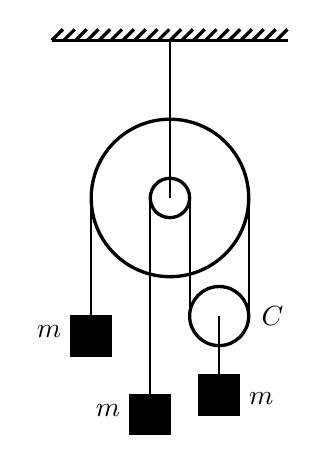
\begin{tikzpicture}[interface/.style={postaction={draw,decorate,decoration={border,angle=45,amplitude=0.2cm,segment length=1.5mm}}},>=latex]
  % \draw[help lines,step=0.5] (0,-2) grid (4,4);  
  \draw[very thick,interface] (0.5,4) -- +(3,0);
  \draw[thick] (2,4) -- +(0,-2);
  \draw[very thick] (2,2) circle (1cm);
  \draw[very thick] (2,2) circle (0.25cm);
  \draw[thick] (1,2) -- +(0,-1.5);
  \draw[thick] (3,2) -- +(0,-1.5);
  \draw[very thick] (3-0.75/2,0.5) circle (0.75/2) node[right=0.4cm] {$C$};
  \draw[thick] (3-0.75/2,0.5) -- +(0,-0.75);
  \filldraw[black,thick] (2.75-0.75/2,-0.25) rectangle +(0.5,-0.5)
  node[above right] {$m$};
  \filldraw[black,thick] (0.75,0.5) rectangle +(0.5,-0.5) node[above=0.3cm,left=0.5cm] {$m$};
  \draw[thick] (1.75,2) -- +(0,-2.5);
  \draw[thick] (2.25,2) -- +(0,-1.5);
  \filldraw[black,thick] (1.5,-0.5) rectangle +(0.5,-0.5) node[above=0.3cm,left=0.5cm] {$m$};
\end{tikzpicture}
}
\taskpic{ Два тела с массами $m_1$ и $m_2$ связаны невесомой нерастяжимой
  нитью, перекинутой через невесомый блок, так, что тело $m_2$ висит,
  а тело $m_1$ лежит на горизонтальной поверхности. К телу $m_1$
  приложена в горизонтальном направлении сила $F$. Найдите ускорения
  тел и силу натяжения нити. Трение отсутствует.  }
{
  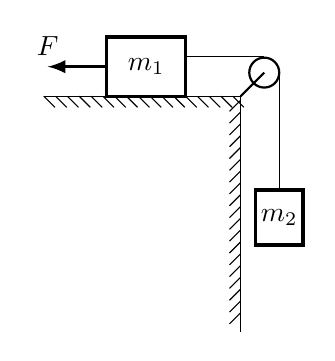
\begin{tikzpicture}[interface/.style={postaction={draw,decorate,decoration={border,angle=-45,amplitude=0.2cm,segment length=1.5mm}}},>=latex]
  \draw[interface] (0.2,4.5) -- ++(2.5,0) -- ++(0,-3);
  \draw[very thick] (1,4.5) rectangle ++(1,0.75) node[midway] {$m_1$};
  \draw[very thick,->] (1,4.5+0.75/2) -- +(-0.75,0) node[above] {$F$}; 
  \draw[thick] (2.7,4.5) -- ++(0.3,0.3) circle (0.19);
  \draw (2,5) -- ++(1,0) ++(0.19,-0.19) -- +(0,-1.5);
  \draw[very thick] (3.19-0.3,5-0.19-1.5) rectangle ++(0.6,-0.7)
  node[midway] {$m_2$};
\end{tikzpicture}
}